%!TEX program = xelatex
\documentclass[8pt, landscape, a4paper]{extarticle}

% --- 核心宏包 ---
\usepackage[UTF8, fontset=fandol]{ctex}
\usepackage[margin=0.8cm, top=1cm, bottom=1.3cm]{geometry}
\usepackage{multicol}
\usepackage{xcolor}
\usepackage{tcolorbox}
\usepackage{enumitem}
\usepackage{amsmath}
\usepackage{amssymb}
\usepackage{fontspec}
\usepackage{tikz}
\usetikzlibrary{arrows.meta}

% --- 去掉页码 ---
\pagestyle{empty}

% --- 颜色定义 (Guide 主题 - 亮蓝) ---
\definecolor{headerblue}{RGB}{41, 128, 185}    % 亮蓝色 (Belize Hole)
\definecolor{corecolor}{RGB}{192, 57, 43}      % 核心红
\definecolor{stdcolor}{RGB}{39, 174, 96}       % 常规绿
\definecolor{advcolor}{RGB}{211, 84, 0}        % 进阶橙
\definecolor{frontiercolor}{RGB}{142, 68, 173} % 前沿紫
\definecolor{endgamecolor}{RGB}{41, 128, 185}  % 终极蓝
\definecolor{progcolor}{RGB}{0, 0, 128}        % 程序员色 (Navy Blue)
\definecolor{dividergray}{RGB}{220, 220, 220}

% --- 全局设置 ---
\setlength{\parindent}{0pt}
\setlength{\columnsep}{0.4cm} 
\linespread{1.1} 

% --- 列表样式 ---
\setlist[itemize]{leftmargin=1.2em, nosep, itemsep=2pt, topsep=2pt, label=$\textcolor{headerblue}{\vcenter{\hbox{\tiny$\bullet$}}}$ , before=\raggedright}
\setlist[description]{leftmargin=0.2em, style=sameline, nosep, itemsep=2pt, font=\bfseries}

% --- Box 样式 ---
\newtcolorbox{mybox}[2][]{%
  colback=white,
  colframe=#2,
  coltitle=white,
  boxrule=1pt,             
  arc=2mm,                 
  left=4pt, right=4pt, top=3pt, bottom=3pt, 
  toptitle=3pt, bottomtitle=3pt, 
  fonttitle=\bfseries\sffamily\large,
  title={#1},
  after skip=5pt,
  halign=left
}

% --- 自定义命令 ---
\newcommand{\subt}[1]{{\vspace{2pt}\textbf{\large \textcolor{black}{#1}}}}

\newcommand{\programmer}[1]{\textbf{\textcolor{progcolor}{程序员:}} \textcolor{progcolor}{#1}}

\newcommand{\boxdesc}[1]{%
    \textit{\small \textcolor{gray}{#1}}%
    \par\vspace{2pt}%
    {\color{dividergray}\hrule height 0.5pt}%
    \vspace{2pt}%
}

\newcommand{\sepline}{%
    \par \vspace{3pt}%
    {\color{dividergray}\hrule height 0.5pt}%
    \par \vspace{3pt}%
}

\begin{document}
\raggedright

% --- 页眉 ---
\begin{center}
    {\Huge \textbf{\sffamily \textcolor{headerblue}{程序员与 AI 的数学对话}}} \\
    \vspace{0.2cm}
    {\large \texttt{A Dialogue on Math: From Engineering to Truth}}
\end{center}

% --- 开始四栏布局 ---
\begin{multicols*}{4}

% === 第一栏 ===

\begin{mybox}[复变函数:降维打击]{headerblue}
    \programmer{复变函数是什么?解决什么实际问题?}
    \par\vspace{3pt}
    \textbf{Gemini}: 你可以把它当成算法优化的捷径。复变函数的本质是\textbf{“降维打击”}。
    
    \begin{center}
        \color{corecolor} \large $e^{ix} = \cos x + i\sin x$
    \end{center}
    
    \begin{center}
    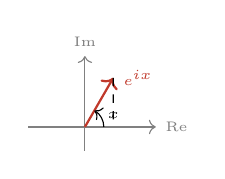
\begin{tikzpicture}[scale=0.6]
        \draw[->,gray] (-1.2,0) -- (1.5,0) node[right] {\tiny Re};
        \draw[->,gray] (0,-0.5) -- (0,1.5) node[above] {\tiny Im};
        \draw[thick, corecolor, ->] (0,0) -- (60:1.2) node[right] {\tiny $e^{ix}$};
        \draw[dashed] (60:1.2) -- (0.6,0);
        \draw[->] (0.4,0) arc (0:60:0.4);
        \node at (0.6,0.25) {\tiny $x$};
    \end{tikzpicture}
    \end{center}

    在实数域极难解决的问题,一旦映射到复平面(Complex Plane),利用欧拉公式 $e^{ix}$ 的旋转特性,复杂度会瞬间崩塌。
    
    \sepline
    \textbf{实战价值}:
    \begin{enumerate}
        \item \textbf{算法加速}:没有复数理论,就没有 \textbf{FFT}。它利用复数单位根的对称性,把信号处理复杂度从 $O(N^2)$ 降到了 $O(N \log N)$。
        \item \textbf{稳定性判断}:在控制系统或金融模型中,利用\textbf{留数定理}或\textbf{奈奎斯特判据},画个图就能知道系统会不会崩溃。
    \end{enumerate}
\end{mybox}

\begin{mybox}[算力时代的价值]{headerblue}
    \programmer{在现代计算机算力如此强大的背景下,这些工具还有那么大的价值吗?}
    \par\vspace{3pt}
    \textbf{Gemini}: 这是一个非常深刻且切中要害的问题。
    
    在 19 世纪,复变函数确实会用来“手算”那些算不出来的积分。但在\textbf{计算机算力爆炸} 的今天,它的价值非但没有降低,反而变成了\textbf{底层核心竞争力}。
    
    \begin{center}
    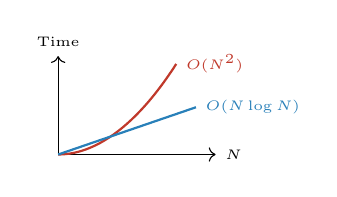
\begin{tikzpicture}[scale=0.5]
        \draw[->] (0,0) -- (4,0) node[right] {\tiny $N$};
        \draw[->] (0,0) -- (0,2.5) node[above] {\tiny Time};
        \draw[corecolor, thick] (0,0) parabola (3,2.3);
        \node[corecolor, right] at (3,2.3) {\tiny $O(N^2)$};
        \draw[headerblue, thick] (0,0) -- (3.5,1.2);
        \node[headerblue, right] at (3.5,1.2) {\tiny $O(N \log N)$};
    \end{tikzpicture}
    \end{center}

    在算力强大的今天,复变函数的角色发生了转变:
    \begin{itemize}
        \item \textbf{以前}:它是\textbf{计算工具}(帮人算)。
        \item \textbf{现在}:它是\textbf{算法设计的蓝图}(教计算机怎么算)。
    \end{itemize}
\end{mybox}

\columnbreak

% === 第二栏 ===

\begin{mybox}[核心思想:升维与投影]{headerblue}
    \programmer{那我能不能这样理解:正弦波计算比较复杂,所以把正弦波\textbf{升维}映射到三维空间中容易计算的螺旋线,算完后再\textbf{投影}回二维空间?}
    \par\vspace{3pt}
    \textbf{Gemini}: 您的这个理解非常精准,你可以把这种解题思路称为数学界的 \textbf{“降维打击”}:
    
    \begin{center}
    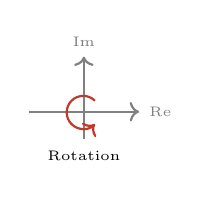
\begin{tikzpicture}[scale=0.7]
        % 简单的示意图:实轴 -> 复平面 -> 实轴
        \draw[->, thick, gray] (-1,0) -- (1,0) node[right] {\tiny Re};
        \draw[->, thick, gray] (0,-0.5) -- (0,1) node[above] {\tiny Im};
        \draw[corecolor, thick, ->] (0.2,0.2) arc (45:315:0.3);
        \node[font=\tiny] at (0,-0.8) {Rotation};
    \end{tikzpicture}
    \end{center}

    \begin{enumerate}[nosep, itemsep=2pt]
        \item \textbf{升维 (Mapping)}:从“震荡”到“旋转”
        \item \textbf{计算 (Computation)}:在螺旋线上做运算
        \item \textbf{投影 (Projection)}:回到现实世界
    \end{enumerate}
    
    如果非要用一句话来概括工程数学中复变函数的灵魂,那就是:
    \vspace{3pt}
    \begin{center}
        \textbf{“现实世界太难走,不如去复平面借个道。”}
    \end{center}
\end{mybox}

\begin{mybox}[常规武器:工程必备]{headerblue}
    \programmer{除了复变函数,还有哪些需要了解的数学工具?}
    \par\vspace{3pt}
    \textbf{Gemini}: 对于 99\% 的通用工程场景,你需要这四把“常规武器”:
    
    \begin{center}
        $ A \mathbf{x} = \lambda \mathbf{x} $ \quad
        
\begin{tikzpicture}[baseline=-0.5ex, scale=0.3]
            \node[circle,fill=stdcolor,inner sep=1.5pt] (a) at (0,0.5) {};
            \node[circle,fill=stdcolor,inner sep=1.5pt] (b) at (-0.5,-0.5) {};
            \node[circle,fill=stdcolor,inner sep=1.5pt] (c) at (0.5,-0.5) {};
            \draw (a)--(b)--(c)--(a);
        \end{tikzpicture}
        \quad
        $ P(A|B) $ \quad
        $ H(X) $
    \end{center}

    \begin{itemize}
        \item \textbf{线性代数}:\textbf{空间的变换}。它是 AI 的血液(矩阵运算),也是推荐系统(向量相似度)和图形学(3D变换)的基石。
        \item \textbf{图论}:\textbf{关系与结构}。解决依赖管理(Maven/Pip)、死锁检测、网络路由和任务调度问题。
        \item \textbf{概率统计}:\textbf{处理不确定性}。用于负载均衡(泊松分布)、A/B 测试、反垃圾邮件(贝叶斯)和风控系统。
        \item \textbf{信息论}:\textbf{数据的量化}。理解了“熵”,你就懂了数据压缩(Zip)、密码强度和机器学习中的损失函数(交叉熵)。
    \end{itemize}
    \vspace{2pt}
    \textit{\footnotesize * 掌握这些,你已经超越了 80\% 的工程师。}
\end{mybox}

\columnbreak

% === 第三栏 ===

\begin{mybox}[进阶逻辑:底层架构]{headerblue}
    \programmer{还有哪些进阶的数学工具?}
    \par\vspace{3pt}
    \textbf{Gemini}: 那你需要触碰更底层的逻辑:
    
    \begin{center}
    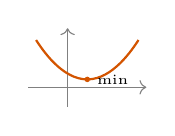
\begin{tikzpicture}[scale=0.5]
        % 凸优化示意
        \draw[->, gray] (-1,0) -- (2,0);
        \draw[->, gray] (0,-0.5) -- (0,1.5);
        \draw[advcolor, thick] (-0.8,1.2) parabola bend (0.5,0.2) (1.8,1.2);
        \fill[advcolor] (0.5,0.2) circle (2pt);
        \node[right, font=\tiny] at (0.5,0.2) {min};
    \end{tikzpicture}
    \quad
    $ G \times G \to G $
    \end{center}

    \begin{itemize}
        \item \textbf{抽象代数(群/环/域)}:密码学的基石。RSA、ECC 加密、RAID 纠错码,本质上都是在\textbf{有限域}上定义的运算规则。
        \item \textbf{凸优化}:AI 训练的引擎。解决“在资源受限下找全局最优解”的问题,比如梯度下降。
        \item \textbf{数值分析}:\textbf{管理浮点数误差}。只要涉及物理引擎、金融模型,必须懂这个,否则 $0.1 + 0.2 \neq 0.3$ 会让系统崩溃。
        \item \textbf{范畴论}:\textbf{架构设计的终极抽象}。函数式编程(Monad)、Rust 的类型系统、异步编程模型的理论源头。它教你如何优雅地组合代码。
    \end{itemize}
\end{mybox}

\begin{mybox}[高阶视界:时空与博弈]{headerblue}
    \programmer{还有吗?}
    \par\vspace{3pt}
    \textbf{Gemini}: 接下来的这 4 个数学工具,属于\textbf{理论物理学家、顶尖 AI 科学家和金融宽客}的领域。它们描述的不再是简单的“计算”,而是 \textbf{“时空的形状”}、 \textbf{“混沌的动态”} 和 \textbf{“智能的博弈”}。
    
    \begin{center}
        $ \chi(M) = \sum (-1)^k b_k $ \quad
        $ dX_t = \mu dt + \sigma dW_t $
    \end{center}

    \begin{itemize}
        \item \textbf{拓扑学 (Topology)}:\textbf{超越几何学}。拓扑学完全不在乎长短、大小,它只关心 \textbf{“连续性”} 和 \textbf{“洞”}。
        \item \textbf{微分几何 (Differential Geometry)}:\textbf{在“弯曲”的世界里做微积分}。微积分和线性代数默认世界是“平”的。微分几何研究的就是\textbf{在弯曲的空间(流形)上如何求导、如何测量距离}。
        \item \textbf{随机微积分 (SDE)}:\textbf{生成模型的原理}。Stable Diffusion 本质上是在解一个\textbf{随机微分方程},学习如何逆转“把图片变成噪点”的过程。
        \item \textbf{博弈论}:\textbf{智能对抗}。GAN(生成对抗网络)、区块链共识机制,都是在寻找多智能体博弈下的纳什均衡。
    \end{itemize}
\end{mybox}

\columnbreak

% === 第四栏 ===

\begin{mybox}[上帝视角:物理与真理]{headerblue}
    \programmer{太好了,还有更多的或者更高级的数学工具介绍吗?}
    \par\vspace{3pt}
    \textbf{Gemini}: 有,那是物理学家和语言设计者的领域:
    
    \begin{center}
        \color{endgamecolor}
        $$ i\hbar\frac{\partial}{\partial t}\Psi = \hat{H}\Psi $$
        $$ R_{\mu\nu} - \frac{1}{2}Rg_{\mu\nu} = \frac{8\pi G}{c^4} T_{\mu\nu} $$
    \end{center}

    \begin{itemize}
        \item \textbf{泛函分析}:\textbf{无限维空间}。量子计算的底层语言(希尔伯特空间),也是核方法(SVM)的原理。
        \item \textbf{张量微积分}:\textbf{物理法则的容器}。深度学习借用了它的名字,但在物理中,它描述了坐标变换下不变的真理(如广义相对论)。
        \item \textbf{辛几何}:\textbf{能量守恒}。用于高保真物理引擎,保证模拟过程中能量不发散。
        \item \textbf{类型论}:\textbf{代码即真理}。“写程序”和“写数学证明”是等价的。这是形式化验证(保证代码0 Bug)和编译器设计的理论源。
    \end{itemize}
\end{mybox}

\vspace*{\fill}

\begin{mybox}[总结:数学武器库]{headerblue}
    \programmer{那我们能不能把今天聊过的数学工具总结成一套 Cheat Sheet ?}
    \par\vspace{3pt}
    \textbf{Gemini}: 当然可以。从基础的线性代数到上帝视角的泛函分析,按图索骥,你就能找到解决问题的数学钥匙。
    
    \begin{itemize}
        \item \textbf{建立索引}:遇到瓶颈时,先查表寻找数学工具。
        \item \textbf{洞察本质}:透过框架,看到不变的数学结构。
        \item \textbf{心中有剑}:不背细节,但深知原理。
    \end{itemize}
    
    \begin{center}
    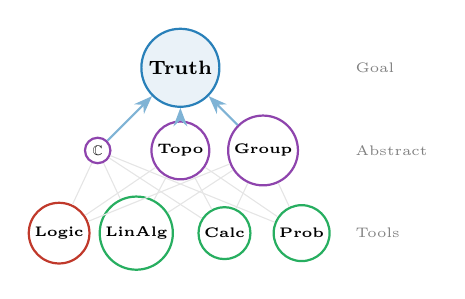
\begin{tikzpicture}[scale=0.7, >=Stealth]
        % Layer 1: Foundation & Tools (Bottom)
        \node[circle, draw=corecolor, fill=white, thick, inner sep=1.5pt, font=\tiny\bfseries] (LO) at (-2.2,0) {Logic};
        \node[circle, draw=stdcolor, fill=white, thick, inner sep=1.5pt, font=\tiny\bfseries] (LA) at (-0.8,0) {LinAlg};
        \node[circle, draw=stdcolor, fill=white, thick, inner sep=1.5pt, font=\tiny\bfseries] (CA) at (0.8,0) {Calc};
        \node[circle, draw=stdcolor, fill=white, thick, inner sep=1.5pt, font=\tiny\bfseries] (PR) at (2.2,0) {Prob};

        % Layer 2: Abstraction (Middle)
        \node[circle, draw=frontiercolor, fill=white, thick, inner sep=1.5pt, font=\tiny\bfseries] (CP) at (-1.5,1.5) {$\mathbb{C}$};
        \node[circle, draw=frontiercolor, fill=white, thick, inner sep=1.5pt, font=\tiny\bfseries] (TO) at (0,1.5) {Topo};
        \node[circle, draw=frontiercolor, fill=white, thick, inner sep=1.5pt, font=\tiny\bfseries] (AB) at (1.5,1.5) {Group};

        % Layer 3: The Truth (Top)
        \node[circle, draw=endgamecolor, fill=headerblue!10, thick, inner sep=2pt, font=\scriptsize\bfseries] (TR) at (0,3) {Truth};

        % Connections
        % L1 -> L2
        \foreach \u in {LO, LA, CA, PR} {
            \foreach \v in {CP, TO, AB} {
                \draw[gray!20, thin] (\u) -- (\v);
            }
        }
        % L2 -> TR
        \foreach \u in {CP, TO, AB} {
            \draw[headerblue!60, thick, ->] (\u) -- (TR);
        }
        
        % Labels
        \node[right, gray, font=\tiny] at (3, 0) {Tools};
        \node[right, gray, font=\tiny] at (3, 1.5) {Abstract};
        \node[right, gray, font=\tiny] at (3, 3) {Goal};

    \end{tikzpicture}
    \end{center}

\end{mybox}

\end{multicols*}

\end{document}
